\chapter{Przegląd istniejących zbiorów}
Zbiory danych w kontekście uczenia maszynowego stanowią fundamentalny element, wymagany do podejmowania wszelakich problemów. Mają bardzo duży wpływ na skuteczność każdego modelu i z tego powodu przed przystąpieniem do tworzenia polskich odpowiedników zostało poświęcone wiele wysiłku na przeanalizowanie zbiorów istniejących.

Na początku bieżącego rozdziału dokładnie przedstawiony zostanie zbiór \code{Spider}, ze szczególnym zwróceniem uwagi na jego format, którego polskie zbiory będą musiały przestrzegać. W kolejnej części nastąpi przegląd zbiorów do niego pokrewnych, czyli takich, które powstały na fundamencie baz danych \code{Spider} i również odegrały w niniejszej pracy istotną rolę. Na koniec nastąpi dogłębna analiza istniejących tłumaczeń zbioru \code{Spider}, aby dokonać świadomych decyzji podczas tworzenia tłumaczenia polskiego.

\section{Angielski Spider}
\code{Spider} to przede wszystkim zbiór danych przeznaczony do zadania \code{Text-to-SQL}, ale również wyzwanie z publicznie dostępnym rankingiem\furl{https://yale-lily.github.io/spider}, które pozwala konkurować badaczom w tworzeniu coraz lepszych modeli oraz śledzić czynione postępy na przestrzeni czasu.

Na zbiór składa się \numprint{10181} próbek, które są podzielone na trzy części: treningową, walidacyjną (zwaną również deweloperską) oraz testową. Ta ostatnia nie jest jednak powszechnie dostępna i sprawność swojego modelu można uzyskać na niej jedynie poprzez wysłanie go do wyzwania. Daje to pewność, że przypuszczalnie dobre wyniki wysyłanych modeli nie są skutkiem przypadkowego, ani celowego włączenia próbek testowych do zbioru treningowego, czyli zjawiska tak zwanego wycieku danych. Brak swobodnego dostępu do części testowej sprawia, że w praktyce część walidacyjna często przejmuję jej rolę.

Próbki ze zbioru \code{Spider} opierają się na 200 bazach danych, które są bardzo różnorodne, ponieważ obejmują 138 domen, takich jak uczelnie, programy telewizyjne, czy rząd. W niektórych przypadkach ta sama tematyka poruszana jest przez kilka baz danych, co tłumaczy fakt, że jest ich więcej niż samych domen. Bardzo ważne jest to, że bazy są rozdzielone na poszczególne części zbioru. Między innymi żadna baza wykorzystywana w części treningowej nie jest używana w części walidacyjnej ani testowej. Wymusza to na uczonych za pomocą tego zbioru modelach posiadanie umiejętności uogólniania na nowe domeny.

\subsection{Format zbioru}

Wiele istniejących modeli wykorzystuję zbiór \code{Spider} ze względu na jego unikatowość i co za tym idzie, reprezentowany przez niego format stał się w pewien sposób standardem. Nie jest to prosty format tabelaryczny, jak to wygląda w postaci wielu innych zbiorów, lecz składają się na niego cztery jakościowo różne komponenty. Są to przykłady, poprawne zapytania SQL (ang. gold queries), schemat baz danych oraz same bazy. Nieco uproszczona struktura plików zbioru została przedstawiona na rysunku \ref{fig:spider-structure} 

\begin{figure}[ht]
  \centering
    \begin{forest}
      for tree={
        inner sep=0pt,l=10pt,l sep=10pt,
        font=\ttfamily,
        grow'=0,
        child anchor=west,
        parent anchor=south,
        anchor=west,
        calign=first,
        edge path={
          \noexpand\path [draw, \forestoption{edge}]
          (!u.south west) +(7.5pt,0) |- node[fill,inner sep=1.25pt] {} (.child anchor)\forestoption{edge label};
        },
        before typesetting nodes={
          if n=1
            {insert before={[,phantom]}}
            {}
        },
        fit=band,
        before computing xy={l=15pt},
      }
    [Spider
      [database
        [db1]
        [db2]
        [...]
      ]
      [dev.json]
      [train\_spider.json]
      [train\_others.json]
      [dev\_gold.sql]
      [train\_gold.sql]
      [tables.json]
    ]
    \end{forest}
\caption{Struktura plików zbioru \code{Spider}}
  \label{fig:spider-structure}
\end{figure}

\subsubsection{Próbki (\hcode{dev.json}, \hcode{train\_spider.json}, \hcode{train\_others.json})} 
Próbki przechowywane są w formacie JSON i podzielone zostały na trzy pliki. W \code{dev.json} znajdują się te odpowiadające zbiorowi walidacyjnemu, natomiast w plikach \code{train\_spider.json} oraz \code{train\_others.json} umieszczono próbki treningowe. Są one rozdzielone dodatkowo na dwa pliki, ponieważ w pierwszym twórcy zbioru umieścili swoje autorskie przykłady, natomiast w drugim te wyselekcjonowane z już istniejących zbiorów. Przykładowa próbka została przedstawiona na listingu \ref{lst:spider-sample}.

\begin{minipage}{\linewidth}
\lstinputlisting[
style=json,
caption=Przykładowa próbka ze zbioru \code{Spider},
label={lst:spider-sample},
]{listings/spider_sample.json}
\end{minipage}

Znaczenie poszczególnych atrybutów próbki jest następujące:\nobreakpar
\begin{itemize}
    \item \textbf{\code{db\_id}} -- identyfikator bazy danych,
    \item \textbf{\code{question}} -- pytanie w języku naturalnym,
    \item \textbf{\code{question\_toks}} -- pytanie podzielone na tokeny,
    \item \textbf{\code{query}} -- zapytanie SQL,
    \item \textbf{\code{query\_toks}} -- zapytanie SQL podzielone na tokeny,
    \item \textbf{\code{query\_toks\_no\_value}} -- zapytanie SQL podzielone na tokeny, ale z zamaskowanymi wszystkimi wartościami, a dokładnie zastąpionymi tekstem \code{value},
    \item \textbf{\code{sql}} -- skomplikowany obiekt JSON będący sparsowanym zapytaniem SQL, pozwalający na szybkie liczenie metryk i wydobywanie różnych fragmentów zapytania.
\end{itemize}

\subsubsection{Poprawne zapytania SQL (\code{dev\_gold.sql}, \code{train\_gold.sql})}
Poprawne zapytania SQL, zgodnie z powyższym opisem, stanowią jeden z atrybutów próbek, lecz poza tym są również wyciągnięte do dwóch osobnych plików \code{dev\_gold.sql} oraz \code{train\_gold.sql}, które odpowiadają części walidacyjnej oraz treningowej. W każdej linii tych plików, jak przedstawiono na listingu \ref{lst:spider-gold}, umieszczone jest poprawne zapytanie SQL oraz identyfikator bazy danych oddzielony od zapytania znakiem tabulacji.

\begin{minipage}{\linewidth}
\lstinputlisting[
style=sql,
caption=Fragment pliku \code{dev\_gold.json} zawierającego poprawne zapytania SQL,
label={lst:spider-gold}
]{listings/spider_gold.txt}
\end{minipage}

\subsubsection{Schemat (\code{tables.json})}
Plik \code{tables.json}, którego fragment został przedstawiony na listingu \ref{lst:spider-tables}, opisuję strukturę każdej zawartej w zbiorze \code{Spider} bazy danych. Obejmuję to wskazanie nazw wszystkich tabel i kolumn, typów kolumn, kluczy podstawowych oraz relacji tworzonych przez klucze obce. 

\begin{minipage}{\linewidth}
\lstinputlisting[
style=json,
caption=Fragment pliku \code{tables.json} opisujący schemat pojedynczej bazy danych,
label={lst:spider-tables},
]{listings/spider_tables.json}
\end{minipage}

Znaczenie poszczególnych atrybutów obiektu opisującego schemat bazy danych jest następujące:\nobreakpar
\begin{itemize}
    \item \textbf{\code{db\_id}} -- identyfikator bazy danych,
    \item \textbf{\code{table\_names\_original}} -- nazwy tabel występujących w bazie,
    \item \textbf{\code{table\_names}} -- naturalne odpowiedniki nazw tabel występujących w bazie,
    \item \textbf{\code{column\_names\_original}} -- sekwencja dwuelementowych list zawierających kolejno numer porządkowy tabeli oraz nazwę zawartej w niej kolumny,
    \item \textbf{\code{column\_names}} -- tak jak wyżej, lecz z naturalnymi odpowiednikami nazw kolumn,
    \item \textbf{\code{column\_types}} -- typy danych posiadane przez wyżej wymieniane kolumny,
    \item \textbf{\code{primary\_keys}} -- numery porządkowe kolumn będących kluczami podstawowymi,
    \item \textbf{\code{foreign\_keys}} -- sekwencja dwuelementowych list zawierających kolejno numer porządkowy kolumny będącej kluczem obcym oraz numer porządkowy kolumny będącej powiązanym kluczem podstawowym.
\end{itemize}

Warto zwrócić uwagę na fakt, że w pliku schematu, oprócz oryginalnie występujących w bazie nazw tabel i kolumn, znajdują się również ich odpowiedniki w języku naturalnym. Oznacza to, że nazwy składające się z kilku słów i zapisywane oryginalnie za pomocą różnych konwencji, takich jak Camel Case (np. \code{playerName}), Snake Case (np. \code{player\_name}), czy Pascal Case (np. \code{PlayerName}) są zamieniane na naturalną postać, czyli słowa odseparowane spacjami. Poza tym część oryginalnie skrótowych nazw jest rozwijana do bardziej zrozumiałej postaci. Stanowi to dodatkową informację, która nie jest dostępna w samych bazach danych.

\subsubsection{Bazy danych (\code{database/*})}
Ostatnim komponentem zbioru \code{Spider} jest katalog \code{database} zwierający szereg podkatalogów o nazwach odpowiadających identyfikatorom baz danych. Wewnątrz każdego z tych podkatalogów umieszczona jest baza danych \code{SQLite} oraz opcjonalnie dodatkowe pliki, takie jak skrypt SQL pozwalający zbudować daną bazę od zera. Większość baz, z nielicznymi wyjątkami, jest wypełniona danymi. Jest to istotne, ponieważ duża część nowoczesnych algorytmów opiera się na tych danych, by generowane zapytania SQL były dokładniejsze.

\section{Angielskie zbiory pokrewne} \label{text:related-datasets}
Jedną z ważniejszych zasług zbioru \code{Spider} jest zgromadzenie pokaźnej liczby baz danych pochodzących z bardzo różnych domen. Było to trudne, ponieważ stanowią informacje poufne dla wykorzystujących je firm i niewielka ich liczba jest dostępna w sieci. Nic więc dziwnego, że na fundamencie baz danych \code{Spider} powstało kilka kolejnych zbiorów. Doskonałym tego przykładem są zbiory \code{CoSQL} \mycite{cosql} oraz \code{SParC} \mycite{sparc}, gdzie zachowano te same bazy, lecz stworzone zostały całkowicie nowe przykłady. Pojawiło się również odmienne podejście polegające na skonstruowaniu zbiorów pochodnych poprzez dokonanie w próbkach ze zbioru \code{Spider} pewnych ukierunkowanych modyfikacji, czego przykładem są zbiory \code{Spider-Syn} \mycite{Gan2021spidersyn}, \code{Spider-DK} \mycite{Gan2021spiderdk}, czy \code{Dr.Spider} \mycite{Chang2023}.

Jako że część ze wspomnianych powyżej zbiorów pokrewnych do zbioru \code{Spider} odegrało istotną rolę w dalszej części pracy to zostaną one pobieżnie opisane w poniższych sekcjach.

\subsection{Spider-Syn}
\code{Spider-Syn} \mycite{Gan2021spidersyn} jest zbiorem danych powstałym ze zbioru \code{Spider} poprzez zmodyfikowanie próbek w taki sposób, aby ograniczyć dosłowne wymienianie w pytaniach nazw kolumn, tabel i wartości z baz danych. Odzwierciedla to scenariusz w którym z interfejsu tekstowego do bazy korzysta osoba, która dokładnie jej nie zna, więc często posługuje się mimowolnie synonimami. Przykładowa próbka została przedstawiona na listingu \ref{lst:spider-syn-example}. Stworzenie tego typu zbioru było istotne, ponieważ okazało się, że duża część istniejących algorytmów opiera się na powiązywaniu pytania z elementami baz danych poprzez znajdywanie dosłownych powtórzeń i w przedstawionym scenariuszu ich skuteczność radykalnie spada. Zbiór ten posiada część treningową oraz walidacyjną. Można w klasyczny sposób dokonać nauki modeli na części treningowej i ewaluację na części testowej, lecz również popularnym scenariuszem jest trening na zbiorze \code{Spider} i ewaluacja na obu częściach \code{Spider-Syn}.

\begin{minipage}{\linewidth}
\lstinputlisting[
style=json,
caption=Przykład próbki ze zbioru \code{Spider-Syn},
label={lst:spider-syn-example}
]{listings/spider_syn_example.json}
\end{minipage}

\subsection{Spider-DK}
Zbiór danych \code{Spider-DK} \mycite{Gan2021spiderdk} (skrót od ang. Domain Knowledge) został zbudowany na podstawie części testowej \code{Spider} w celu oceny tworzonych modeli pod kątem znajomości wiedzy domenowej. Składa się na niego skromna ilość próbek w liczbie 535, gdzie prawie połowa została wybrana ze zbioru \code{Spider} i przeniesiona bez zmian, a druga połowa powstała poprzez zmodyfikowanie przykładów tak, aby dodać wiedzę domenową. Przykładowa próbka została przedstawiona na listingu \ref{lst:spider-dk-example}. Posiada ona atrybut \code{type}, który wskazuje jeden z pięciu przewidzianych typów wiedzy domenowej. W celu dokładniejszego zrozumienia można odwołać się do artykułu wprowadzającego zbiór \code{Spider-DK}, lecz są one następujące:
\begin{itemize}
    \item \textbf{Typ 1} -- pomijanie wymieniania kolumn,
    \item \textbf{Typ 2} -- proste wnioskowanie,
    \item \textbf{Typ 3} -- synonimy wartości komórek,
    \item \textbf{Typ 4} -- generowanie warunków na podstawie słów spoza wartości komórek,
    \item \textbf{Typ 5} -- wiedza, która łatwo kłóci się z innymi dziedzinami.
\end{itemize}

\begin{minipage}{\linewidth}
\lstinputlisting[
style=json,
caption={Przykład próbki ze zbioru \code{Spider-DK}},
label={lst:spider-dk-example}
]{listings/spider_dk_example.json}
\end{minipage}

\subsection{SParC}
\code{SParC} \mycite{sparc} jest zbiorem danych zawierającym sekwencje przeplatających się ze sobą pytań w języku naturalnym oraz instrukcji SQL otrzymanych w odpowiedzi. Obejmuje \numprint{4298} sekwencji wiadomości, na które składa się łącznie ponad 12 tysięcy pojedynczych pytań. Są one ze sobą powiązane w obrębie konwersacji i wymagają wykorzystania informacji z poprzednich wiadomości, aby poprawnie sformułować żądane zapytanie SQL. Zbiór ten służy więc do nauki modeli rozwiązujących konwersacyjny wariant problemu \code{Text-to-SQL}. Przykładową konwersację z niego pochodzącą przedstawiono na rysunku \ref{fig:sparc-example}. Widać na niej wyraźnie, że kolejne wiadomości bazują na kontekście wprowadzonym przez wiadomości wcześniejsze.

\begin{figure}[ht!]
  \centering
  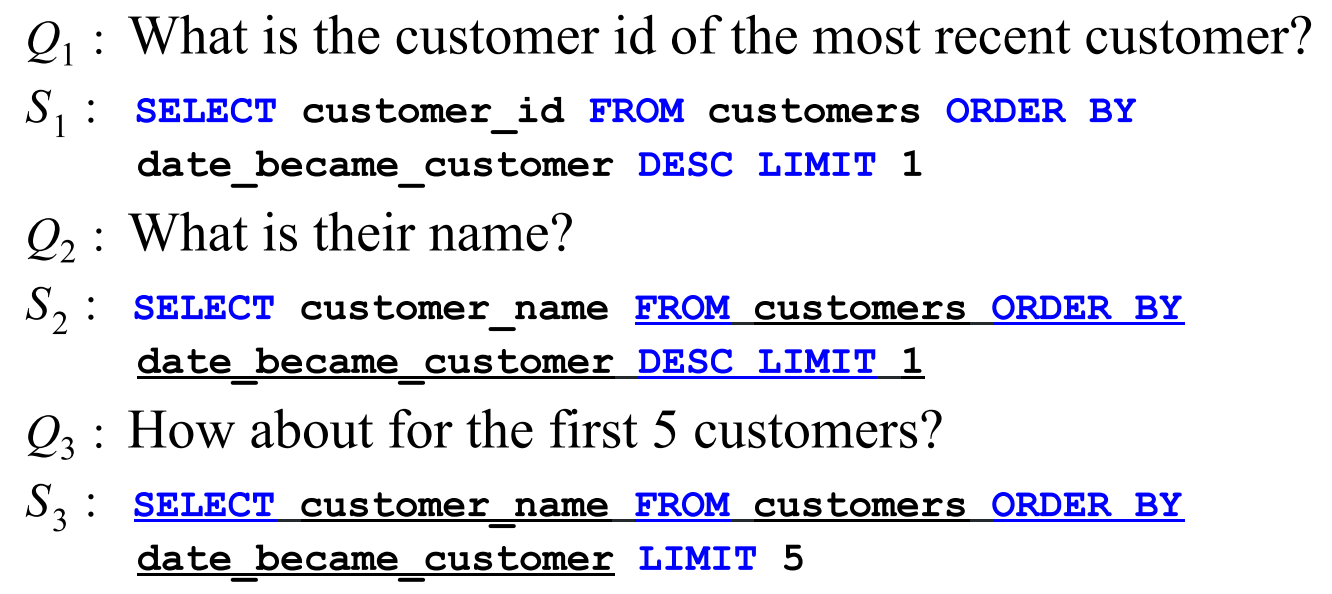
\includegraphics[width=0.6\linewidth]{images/sparc_example.png}
  \caption[Przykładowa konwersacja ze zbioru \code{SParC}]{Przykładowa konwersacja ze zbioru \code{SParC}}
  \source{\code{SParC} \mycite{sparc}}
  \label{fig:sparc-example}
\end{figure}

\subsection{CoSQL}
\code{CoSQL} \mycite{cosql} jest zbiorem w znacznym stopniu podobnym do \code{SParC}, ponieważ zawiera dane o charakterze konwersacyjnym. Został do niego dodany jednak kolejny poziom złożoności, gdyż konwersacje nie stanowią już naprzemiennie powtarzających się pytań i instrukcji SQL, lecz powstały w drodze dalece swobodniejszych symulowanych rozmów pomiędzy zwykłymi użytkownikami a ekspertami SQL. Każdy dialog odtwarza realistyczny scenariusz eksploracji bazy danych, w którym użytkownik zadaje pytania, a ekspert stara się na nie odpowiedzieć, wyjaśniając niejednoznaczne kwestie, czy też informując o pytaniach bez odpowiedzi. Gdy pytania użytkownika dają się sformułować w języku SQL to ekspert tego dokonuje i prezentuje wyniki w sposób pozwalający zachować naturalny przebieg interakcji. Przykładowa rozmowa, która to demonstruje, została przedstawiona na rysunku \ref{fig:cosql-example}. Kompletny zbiór liczy \numprint{30000} dialogów podzielonych na część treningową i testową. Łącznie zawierają \numprint{10000} zapytań.

\begin{figure}[ht!]
  \centering
  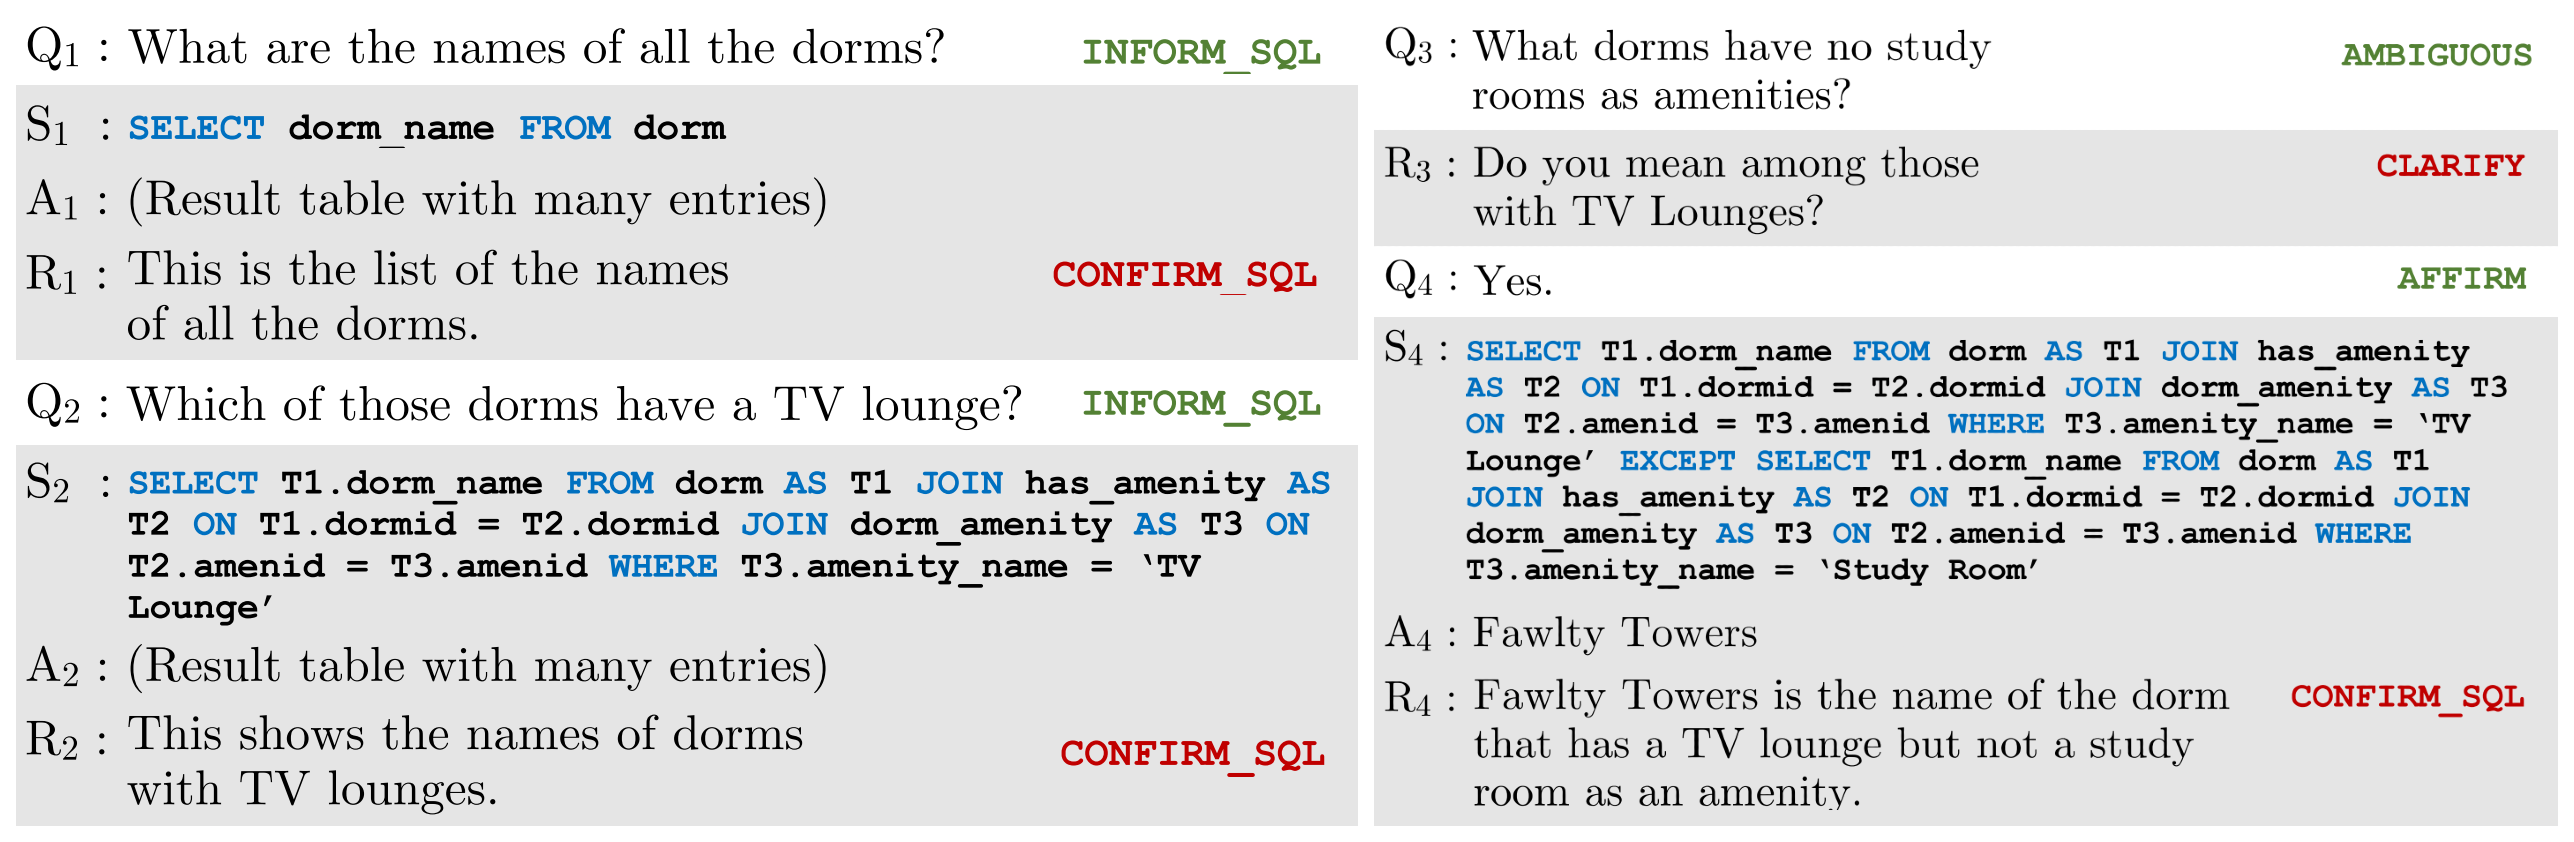
\includegraphics[width=1.0\linewidth]{images/cosql_example.png}
  \caption[Przykładowa konwersacja ze zbioru \code{CoSQL}]{Przykładowa konwersacja ze zbioru \code{CoSQL}}
  \source{\code{CoSQL} \mycite{cosql}}
  \label{fig:cosql-example}
\end{figure}

\section{Tłumaczenia zbioru Spider}
Tak jak zostało zaznaczone we wprowadzeniu, na chwilę obecną wydaje się istnieć pięć publicznie dostępnych zbiorów będących tłumaczeniami \code{Spider}. Cztery spośród nich dokonuje przekładu na konkretny język, a jeden zawiera tłumaczenia na kilka języków. Wspomniane zbiory jednojęzyczne to chiński \code{CSpider}, wietnamski \code{ViText2SQL}, rosyjski \code{PAUQ} oraz nie posiadający nazwy zbiór portugalski. \code{MultiSpider} to natomiast świeży zbiór, bo upowszechniony przez Microsoft w czasie pisanie niniejszej pracy, który zawiera niezależnie opracowane tłumaczenie chińskie, wietnamskie, niemieckie, francuskie, hiszpańskie oraz japońskie. 

Poza publicznie dostępnymi zbiorami danych natrafiono również na wielojęzyczny zbiór \code{XSpider} \mycite{shi-etal-2022-xricl}, który zgodnie z artykułem zawiera między innymi przekłady na język hindi oraz farsi. Jego autorzy twierdzą w artykule, że wszystkie dane umieszczone zostały we wskazanym repozytorium, lecz jest ono całkowicie puste. Zmiana tego stanu jest wątpliwa biorąc pod uwagę fakt, że artykuł ukazał się już ponad dwa lata temu.

Autorzy wymienionych zbiorów, pomimo wspólnego celu, podeszli do zadania na różne sposoby. Celem poniższych sekcji jest przedyskutowanie kluczowych różnic pomiędzy nimi. Jedną z najistotniejszych jest zastosowany rodzaj tłumaczenia. Rozbieżności zaobserwowano również w kwestii tłumaczenia schematu, zawartości baz danych oraz wartości w zapytaniach. Różnice te zostały zestawione w tabeli \ref{tab:spider-trans-diffs} i zostaną dokładnie omówione.


\begin{table}[ht]
    \centering
    \begin{tabular}{|l|c|c|c|c|}
        \hline
        \thead{Zbiór} & 
        \thead{Rodzaj\\tłumaczenia} &
        \thead{Tłumaczenie\\schematu} &
        \thead{Tłumaczenie\\zawartości\\baz danych} &
        \thead{Tłumaczenie\\wartości w\\zapytaniach} \\
        \hline
        \makecell{Chiński\\{\code{CSpider}}} & Manualne & Nie & Nie & Tak \\
        \hline
        \makecell{Wietnamski\\{\code{ViText2SQL}}} & Manualne & Tak & Nie & Tak \\
        \hline
        \makecell{Portugalski\\{\code{Brak Nazwy}}} & Maszynowe & Tak & Nie & Nie \\
        \hline
        \makecell{Rosyjski\\{\code{PAUQ}}} & Manualne & Nie & Częściowo & Tak \\
        \hline
        \makecell{Wielojęzyczny\\{\code{MultiSpider}}} & Manualne & Tak & Nie & Obie wersje \\
        \hline
        \makecell{Wielojęzyczny\\{\code{XSpider}}} & ------ & Nie & ------ & ------ \\
        \hline
    \end{tabular}
    \lcaption{Zestawienie kluczowych różnic pomiędzy tłumaczeniami zbioru \code{Spider}}{Pozioma kreska oznacza brak informacji na dany temat.}
    \label{tab:spider-trans-diffs}
\end{table}

\subsection{Rodzaj tłumaczenia} \label{text:translation-method}
Tłumaczenie maszynowe i manualne to dwa oczywiste podejścia. Pierwsze sprowadza się do wykorzystania gotowych narzędzi, dostępnych najczęściej za pomocą webowych API, takich jak \code{Google Cloud Translation API} \mycite{google-translation-api}, czy \code{DeepL} \mycite{deepl}. Dostępne są również rozwiązania działające offline, czego przykładem jest \code{OpenNMT} \mycite{klein2018opennmt}. Drugie podejście oznacza natomiast ręczne tłumaczenie każdej próbki przez człowieka. Oczywiście tłumaczenie ręczne może być wspomagane przez metodę maszynową, aby ograniczyć się do poprawiania tłumaczeń, zamiast pisania ich od początku.

Największą zaletą tłumaczenia maszynowego jest szybkie uzyskanie przetłumaczonego zbioru. Wiąże się to najczęściej z naliczeniem pewnych kosztów, o których należy wspomnieć, lecz mimo wszystko koszt ten jest niewspółmierny do ceny wynajęcia profesjonalnego ludzkiego tłumacza. Jest on również niewiele znaczący w stosunku do czasu, który trzeba by poświęcić, by dokonać tłumaczenia samemu.

Tłumaczenie maszynowe ma jednak istotne wady -- pomimo że dostępne narzędzia stają się coraz lepsze, to wciąż nie dorównują człowiekowi. Sprawia to, że uzyskiwane zbiory danych są bezsprzecznie niższej jakości. Narzędzia te dokonując tłumaczenia zbioru \code{Spider} nie biorą pod uwagę wielu istotnych elementów, które ludzki adnotator by uwzględnił. Przykładem jest ignorowanie domeny podczas tłumaczenia pytania naturalnego. Ludzki tłumacz pytanie \textit{list all parties} w domenie politycznej przetłumaczy jako \textit{zwróć wszystkie partie}. Tłumacz maszynowy natomiast może to przetłumaczyć jako \textit{zwróć wszystkie imprezy}.

Dotychczasowe tłumaczenia zbioru \code{Spider}, z powodu ograniczeń metody maszynowej, w większości korzystają z ręcznego tłumaczenia zbioru. Jest to prawdą dla rosyjskiego \code{PAUQ}, wietnamskiego \code{ViText2SQL}, chińskiego \code{CSpider} oraz \code{MultiSpider}. Autorzy części z tych manualnie tłumaczonych zbiorów dla porównania dokonali również tłumaczenia maszynowego. Zestawienie wyników osiąganych przez modele trenowane na zbiorach tłumaczonych maszynowo i manualnie zostało przedstawione w tabeli \ref{tab:manual-vs-machine}. Wszystkie wyniki potwierdzają, że tłumaczenie manualne pozwala uzyskać lepsze rezultaty, aczkolwiek w przypadku względnie nowych modeli \code{RAT-SQL} oraz \code{BRIDGE} procentowy spadek skuteczności na zbiorach maszynowych nie jest tak znaczący, jak dla modeli wcześniejszych.

\begin{table}[ht]
    \centering
    \begin{tabular}{|l|l|R{0.15\textwidth}|R{0.15\textwidth}|R{0.15\textwidth}|}
        \hline
        \thead{Zbiór} & \thead{Model} & \thead{Maszynowe} & \thead{Manualne} &
        \thead{Różnica} \\
        \hline
        \code{CSpider} & C-ML & \s7,9 & 12,1 & \s4,1 \\
        \hline
        \code{CSpider} & W-ML & \s0,6 & 10,0 & \s2,4 \\
        \hline
        \code{ViText2SQL} & EditSQL (Vi-Syllable) & 16,8 & 24,1 & \s7,3 \\
        \hline
        \code{ViText2SQL} & EditSQL (Vi-Word) & 17,4 & 30,2 & 12,8 \\
        \hline
        \code{PAUQ} & RAT-SQL & 46,0 & 51,0 & \s5,0 \\
        \hline
        \code{PAUQ} & BRIDGE & 49,0 & 52,0 & \s3,0 \\
        \hline
    \end{tabular}
    \lcaption{Wyniki modeli trenowanych na zbiorach tłumaczonych manualnie i maszynowo}{W trzech ostatnich kolumnach zamieszczono wyrażoną procentowo metrykę Exact Match without values, która zostanie dokładnie opisana w części \ref{section:metrics}. Wyższe wartości metryki oznaczają lepsze rezultaty.}
    \label{tab:manual-vs-machine}
\end{table}

\subsection{Tłumaczenie schematu}
Kolejną kwestią dokonującą podziału wśród istniejących tłumaczeń zbioru \code{Spider} jest obrane podejście co do wynikowego języka schematu baz danych, czyli nazw tabel i kolumn -- mogą być one tłumaczone, albo pozostawione bez zmian w języku angielskim. Drugie podejście jest uzasadnione faktem, że w praktyce, niezależnie od kraju, schemat baz danych jest często utrzymywany w języku angielskim. Ma to takie zalety jak ułatwienie pracy wielonarodowemu zespołowi, czy też uniknięcie problemu ze znakami diakrytycznymi, których wykorzystywanie może być niemożliwe lub utrudnione.

Fakt, że w praktyce nazwy tabel i kolumn zapisywane są w języku angielskim w swoich artykułach wyraźnie podkreślili autorzy tłumaczenia chińskiego, rosyjskiego oraz w pewnym stopniu zbioru \code{XSpider} i z uwagi na to postanowili schematu nie tłumaczyć. Twórcy zbioru wietnamskiego, portugalskiego oraz \code{MultiSpider} postanowili jednak tłumaczenia dokonać, nie przedstawiając dla takiego podejścia specjalnego uzasadnienia.

Należy zauważyć, że reprezentowanie pytań i schematu baz danych w dwóch różnych językach znacząco komplikuje rozwiązywany problem. W wariancie ze wszystkimi komponentami w tym samym języku dość łatwo jest znaleźć powiązania pomiędzy nimi, ponieważ wystarczy przeanalizować ich podobieństwo jako łańcuchów znaków. W przeciwnym przypadku to jednak nie wystarczy -- wykorzystywany model musi przejawiać dodatkowo pewne cechy tłumacza.

Podsumowując, pozostawienie schematu baz danych w języku angielskim jest uzasadnione z praktycznego punktu widzenia, jednak dodatkowo komplikuje zadanie. Zbiór danych z przetłumaczonym schematem, chociaż w dużym stopniu ignoruje aspekt praktyczny, stanowi lepszy odpowiednik oryginalnego zbioru \code{Spider} i pozwala na wykonywanie względem niego bardziej sprawiedliwych porównań.

\subsection{Tłumaczenie zawartości baz danych}
Kolejną niespójnością, jaką można zaobserwować pomiędzy istniejącymi tłumaczeniami zbioru \code{Spider} jest kwestia tłumaczenia zawartości baz danych. Dokonanie takiego tłumaczenia ma istotne zalety przedstawione w kolejnych akapitach, jednak jest to zadanie problematyczne, przez co nie wszyscy autorzy zbiorów się go podjęli.

Większość nowych podejść do problemu generowania SQL analizuje znajdujące się w bazach danych rekordy, aby zwiększyć swoją dokładność. Przykładowo użytkownik systemu może poprosić o zwrócenie populacji Polski, a dwie możliwe odpowiedzi mogłyby zawierać fragmenty \sql{WHERE country = 'PL'} oraz \sql{WHERE country = 'polska'}. Widać tutaj, że schemat bazy nie mówi wszystkiego i bez dostępu do jej zawartości obie odpowiedzi są równie dobre, choć tylko jedna może być poprawna. W celu wytrenowania najlepszych modeli przygotowany zbiór powinien zawierać więc wypełnione bazy danych, a większość istniejących rozwiązań, korzystających z zawartości baz zakłada, że jest ona w tym samym języku co pytania.

Drugim celem wartości w bazach danych jest umożliwienie ewaluacji opracowanych algorytmów \code{Text-to-SQL} za pomocą metryki \code{Execution Accuracy}. Została ona opisana dokładnie w późniejszej części pracy, w sekcji \ref{section:metrics}. Jej skrótowa zasada działania polega na wykonaniu prawidłowych zapytań oraz zapytań wygenerowanych i uznaniu za poprawne tych, które zwróciły te same wyniki. Przetłumaczenie wartości w zapytaniach SQL bez tłumaczenia zawartości baz danych skutkuję tym, że wykonywane zapytania często nie zwracają żadnych wyników, a co za tym idzie, wiele nieprawidłowo wygenerowanych zapytań jest uznawanych omyłkowo za prawidłowe. Podsumowując, różne języki wartości w zapytaniach SQL i wartości w bazach danych skutkują upośledzeniem metryki \code{Execution Accuracy} i zmniejszeniem jej użyteczności.

Modyfikacji zawartości baz danych podjęli się jedynie autorzy tłumaczenia rosyjskiego. Nie tłumaczyli jednak wszystkich wartości, ale tylko te, które wystąpiły w przynajmniej jednym zapytaniu. Powodem, dla którego pozostałe zbiory obyły się bez tłumaczenia jest zapewne duża liczba danych zawartych w bazach i relatywnie niewielkie korzyści wynikające z ich tłumaczenia. Ciekawy pomysł został zastosowany w zbiorze portugalskim oraz \code{MultiSpider}, gdzie zawartość baz danych nie jest tłumaczone, ale wartości w zapytaniach również. Takie podejście pozwala uniknąć obu zarysowanych w powyższych akapitach problemów, ale wydaje się mało praktyczne -- zakłada scenariusz w których w bazach danych o przykładowo portugalskim schemacie przechowywane są dane angielskie.
